\documentclass{standalone}
\usepackage{tikz}
\usetikzlibrary{arrows.meta}

\begin{document}
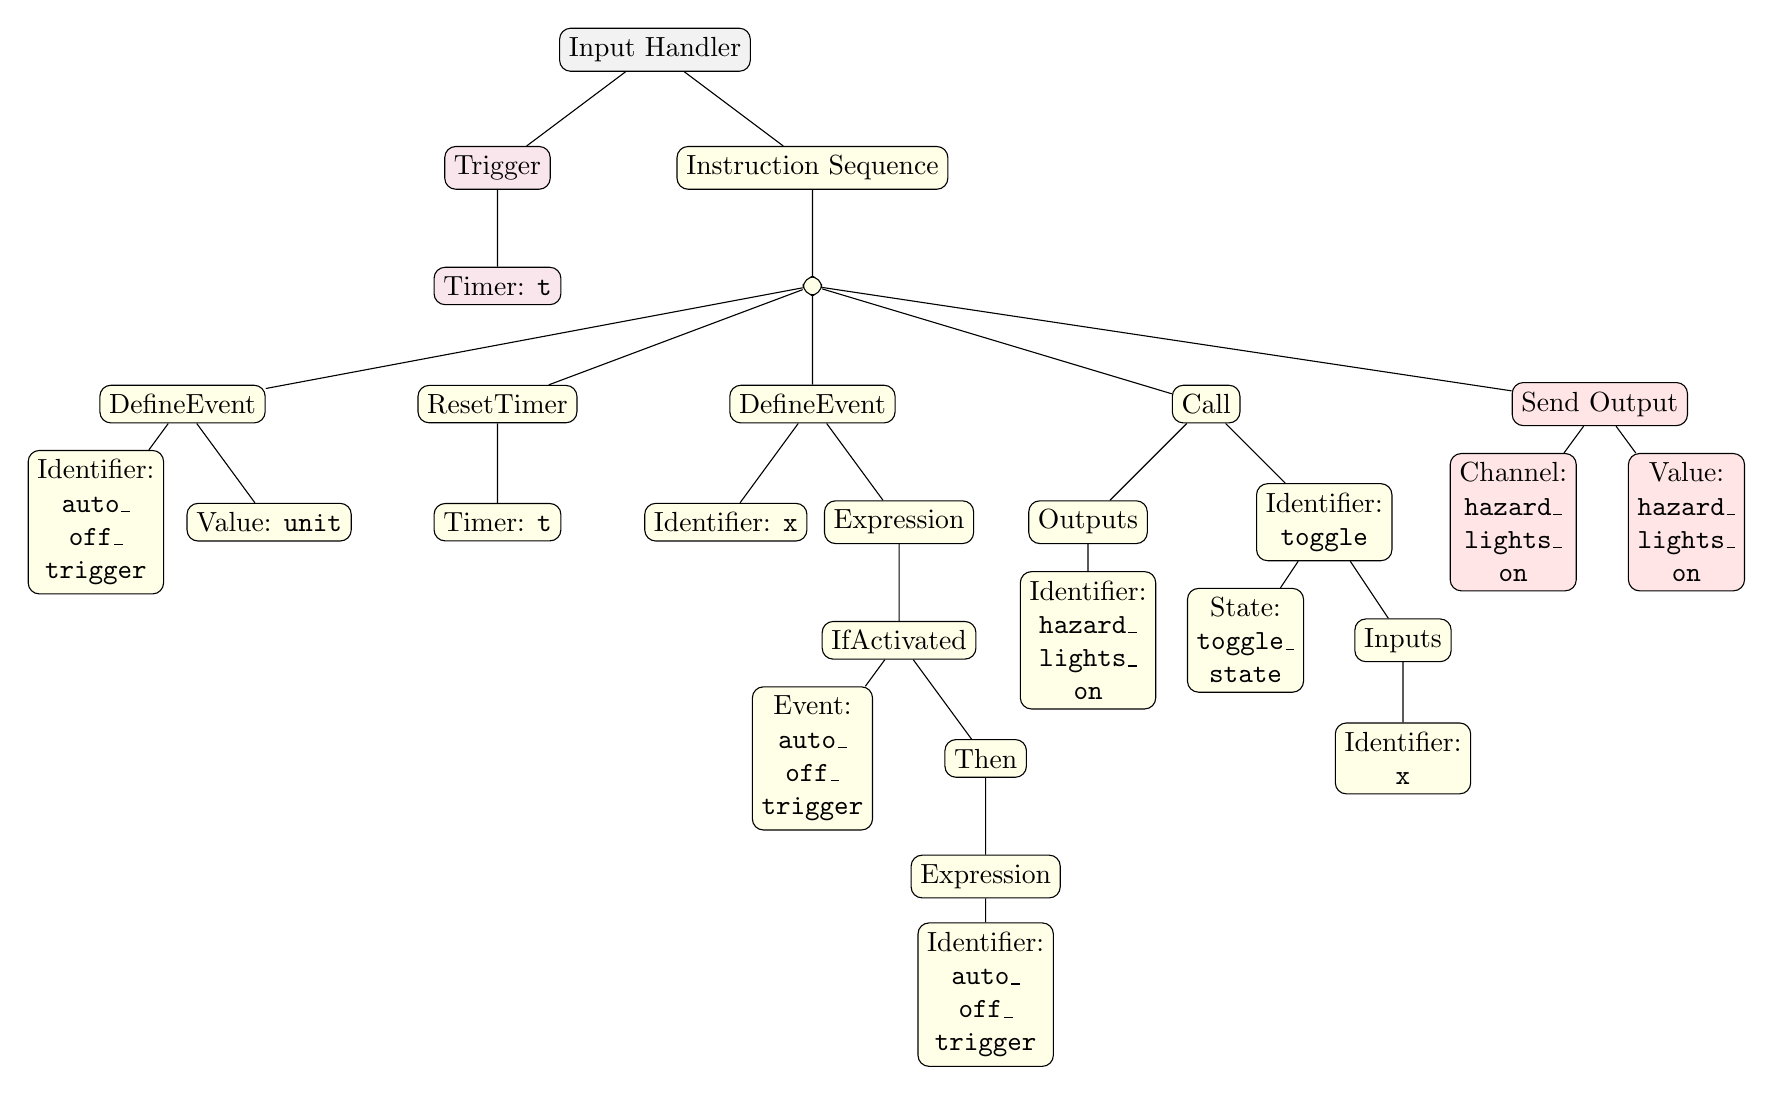
\begin{tikzpicture}[
        level distance=1.5cm, sibling distance=3cm,
        treenode/.style = {rectangle, rounded corners, fill=gray!10, draw, align=center},
        arrow/.style = {-{Stealth[]}}
        ]
        \node[treenode] {Input Handler}
        child [sibling distance=4cm] { node[treenode, fill=purple!10] {Trigger}
                        child { node[treenode, fill=purple!10] {Timer: \texttt{t}} }
                }
        child [sibling distance=4cm] { node[treenode, fill=yellow!10] {Instruction Sequence}
                        child { node[treenode, fill=yellow!10] {}
                                        child [sibling distance=4cm] { node[treenode, fill=yellow!10] {DefineEvent}
                                                        child [sibling distance=2.2cm] { node[treenode, fill=yellow!10] {Identifier:\\\texttt{auto\_}\\\texttt{off\_}\\\texttt{trigger}} }
                                                        child [sibling distance=2.2cm] { node[treenode, fill=yellow!10] {Value: \texttt{unit}} }
                                                }
                                        child [sibling distance=4cm] { node[treenode, fill=yellow!10] {ResetTimer}
                                                        child { node[treenode, fill=yellow!10] {Timer: \texttt{t}} }
                                                }
                                        child [sibling distance=4cm] { node[treenode, fill=yellow!10] {DefineEvent}
                                                        child [sibling distance=2.2cm] { node[treenode, fill=yellow!10] {Identifier: \texttt{x}} }
                                                        child [sibling distance=2.2cm] { node[treenode, fill=yellow!10] {Expression}
                                                                        child { node[treenode, fill=yellow!10] {IfActivated}
                                                                                        child [sibling distance=2.2cm] { node[treenode, fill=yellow!10] {Event:\\\texttt{auto\_}\\\texttt{off\_}\\\texttt{trigger}} }
                                                                                        child [sibling distance=2.2cm] { node[treenode, fill=yellow!10] {Then}
                                                                                                        child [sibling distance=2.2cm] { node[treenode, fill=yellow!10] {Expression}
                                                                                                                        child [sibling distance=2.2cm] { node[treenode, fill=yellow!10] {Identifier:\\\texttt{auto\_}\\\texttt{off\_}\\\texttt{trigger}} }
                                                                                                                }
                                                                                                }
                                                                                }
                                                                }
                                                }
                                        child [sibling distance=5cm] { node[treenode, fill=yellow!10] {Call}
                                                        child [sibling distance=3cm] { node[treenode, fill=yellow!10] {Outputs}
                                                                        child { node[treenode, fill=yellow!10] {Identifier:\\\texttt{hazard\_}\\\texttt{lights\_}\\\texttt{on}} }
                                                                }
                                                        child [sibling distance=3cm] {
                                                                        node[treenode, fill=yellow!10] {Identifier:\\\texttt{toggle}}
                                                                        child [sibling distance=2cm] { node[treenode, fill=yellow!10] {State:\\\texttt{toggle\_}\\\texttt{state}} }
                                                                        child [sibling distance=2cm] { node[treenode, fill=yellow!10] {Inputs}
                                                                                        child { node[treenode, fill=yellow!10] {Identifier:\\\texttt{x}} }
                                                                                }
                                                                }
                                                }
                                        child [sibling distance=5cm] { node[treenode, fill=red!10] {Send Output}
                                                        child [sibling distance=2.2cm] { node[treenode, fill=red!10] {Channel:\\\texttt{hazard\_}\\\texttt{lights\_}\\\texttt{on}} }
                                                        child [sibling distance=2.2cm] { node[treenode, fill=red!10] {Value:\\\texttt{hazard\_}\\\texttt{lights\_}\\\texttt{on}} }
                                                }
                                }
                };
\end{tikzpicture}
\end{document}